\begin{figure*}[t]
\centering
        \begin{subfigure}[b]{0.32\textwidth}
                \centering
                \includegraphics[width=\textwidth]{3_PKN_numerical/accuracy/eps_3.eps}
        \end{subfigure}
        \begin{subfigure}[b]{0.32\textwidth}
                \centering
                \includegraphics[width=\textwidth]{3_PKN_numerical/accuracy/eps_4.eps}
        \end{subfigure}
        \begin{subfigure}[b]{0.32\textwidth}
                \centering
                \includegraphics[width=\textwidth]{3_PKN_numerical/accuracy/eps_5.eps}
        \end{subfigure}
        \begin{picture}(0,0)(490,-105)
        \put(50,-15){$\varepsilon=10^{-3}$}     \put(215,-15){$\varepsilon=10^{-4}$} \put(380,-15){$\varepsilon=10^{-5}$}
        \put(3,10){a)} \put(168,10){b)} \put(335,10){c)}
        \put(3,-33){$\delta f$}      \put(165,-33){$\delta f$} \put(330,-33){$\delta f$}
        \put(80,-110){$N$}    \put(245,-110){$N$} \put(413,-110){$N$}
        \end{picture}
\caption{Maximal relative errors of the solutions computed in different variables $\delta w$, $\delta U$ and $\delta \Omega$, for various number of the grid points $N$
in case of the nonuniform mesh $x^{(II)}$ ($\delta=2$). Different values of $\varepsilon$ have been considered. All computations were performed for the benchmark $q_l^{(1)}$ for
$Q_l/q_0=0.9$. Solutions $U_l$ and $U_n$ obtained by unitization of the linear and nonlinear regularized conditions (\ref{expan_3}) and (\ref{expan_4}), respectively}
\label{fig:err_N_plots}
\end{figure*}


In this section, we analyze the accuracy of computations by the solvers based on different dynamic systems corresponding to the respective dependent variables.
To solve the systems, we use MATLAB ode15s subroutine utilizing a version of the Runge-Kutta method dedicated for stiff dynamic systems.

Before we compare different approaches in terms of their accuracy, let us recall two alternative ways
to define the regularized boundary condition at the end point
$x=1-\varepsilon$. The first one is based on the
$\varepsilon$-regularization technique, as it was defined in
\cite{Linkov_4} (see also \cite{MWL}).
The second approach to formulate the regularized condition is
to take into account the first two terms of asymptotics as described in
section \ref{Rbc} (compare equations: \eqref{expan_1} and
\eqref{BC_N}).
Finally, in the case of $U$, this condition may be implemented in the non-linear form  (\ref{expan_4}).
One can expect that the two term conditions would have a clear
advantage, at least in cases when the solution smoothness near the
crack tip  deteriorates due to the singularity of the leak-off
function.




The results of the computations presented in
Table~\ref{table_UUU} confirm such a prediction. We compare only conditions for $U$, as originally the $\varepsilon$-regularization technique was introduced for this variable.  Indeed, the relative errors
of the solutions $\delta U_l$ or $\delta U_n$ are at least one
order of magnitude lower than that in the case of $\delta U_*$,
corresponding to the formulation based on \eqref{L3}.\footnote{
Here and everywhere later, by $\delta f$ we understand the maximal value of the relative
error of the function $f$ over all discretized independent variables ($\delta f\equiv \|\delta f\|_\infty$).}
Surprisingly, for the variants of the non-singular leak-off function, the improvement
is even more pronounced (especially for a uniform mesh).



\begin{table}
\centering
\begin{tabular}{c c|c@{}|c@{}|c@{}|c@{}|c@{}|c@{}|}
\cline{3-8}
& & \multicolumn{6}{c|}{Comparison of conditions (\ref{L3}), (\ref{expan_3}), (\ref{expan_4})}\\ \cline{3-8}
\cline{3-8}
& & \multicolumn{3}{c|}{$q_l^{(1)} \quad Q_l/q_0=0.9$} & \multicolumn{3}{c|}{$q_l^{(3)} \quad Q_l/q_0=0.5$} \\ \cline{2-8}
& \multicolumn{1}{|c|}{$\epsilon=$} & $10^{-2}$ & $10^{-4}$  & $10^{-6}$ &  $10^{-2}$ &  $10^{-4}$ &  $10^{-6}$ \\ \cline{1-8}
\multicolumn{1}{|c}{\multirow{2}{*}{$\delta U_*$}} & \multicolumn{1}{|c|}{$x^{(I)}$}
 &1.6e-1&1.4e-1&1.3e-1&6.1e-3&3.7e-3&3.7e-3
 \\ \cline{2-8} \multicolumn{1}{|c}{} & \multicolumn{1}{|c|}{$x^{(II)}$}
&1.4e-1&7.6e-2&6.3e-2&4.5e-3&9.3e-5&8.9e-5
 \\ \cline{1-8}
\multicolumn{1}{|c}{\multirow{2}{*}{$\delta U_l$}} & \multicolumn{1}{|c|}{$x^{(I)}$}
 &5.0e-2&1.4e-2&1.7e-2&1.2e-5&1.1e-5&1.1e-5
 \\ \cline{2-8} \multicolumn{1}{|c}{} & \multicolumn{1}{|c|}{$x^{(II)}$}
&5.0e-2&1.7e-3&2.0e-3&4.9e-5&8.2e-5&8.7e-5
 \\ \cline{1-8}
\multicolumn{1}{|c}{\multirow{2}{*}{$\delta U_n$}} & \multicolumn{1}{|c|}{$x^{(I)}$}
 &4.4e-2&1.2e-2&1.3e-2&2.2e-5&1.3e-5&1.3e-5
 \\ \cline{2-8} \multicolumn{1}{|c}{} & \multicolumn{1}{|c|}{$x^{(II)}$}
&4.4e-2&9.9e-4&1.8e-3&4.2e-5&8.2e-5&8.7e-5
 \\ \cline{1-8}
\end{tabular}
\caption{Comparison of the accuracy of the solution of dynamical system based on variable $U$.
The results depicted by $U_*$ refer to the regularized boundary condition  based on one asymptotic term, while those denoted by $U_l$ and $U_n$
correspond to two terms approximation (linear (\ref{expan_3}) and nonlinear (\ref{expan_4}), respectively).
Other problem parameters: $N=100$, $\delta=2$ for the mesh $x^{(II)}$.}
\label{table_UUU}
\end{table}

%\vspace{-4mm}


We also made the computations for three different benchmarks reported in \citet{MWL}. They correspond to the
leak-off function vanishing near the crack tip. It turned out that computational error corresponding to the modified form of the regularized conditions (based on two terms of asymptotics)
was always two orders of magnitude lower than that reported in the previous paper.

On the other hand, there is no difference observed between the solutions $\delta U_l$ but $\delta U_n$
at least for those two benchmarks and the choice of the parameters ($N=100$). However, as we will show  later,
for large numbers of nodal points, or more severe leak-off function relationship ($Q_l/q_0\sim1$),
the nonlinear formulation of the condition clearly manifests its advantage.

From now on only the regularized conditions based on two asymptotic terms \eqref{BC_N} will be utilized.
Additionally, for variable $U$, two different forms, linear
(\ref{expan_3}) and nonlinear (\ref{expan_4}), will be adopted.
For $w$ and $\Omega$ two  formulations, (\ref{L4}) and \eqref{L5}, which are equivalent
to the condition \eqref{L3} could not compete with
their more accurate analogue \eqref{BC_N} in terms of solution accuracy and will not be considered.




Graphs presented in Fig.~\ref{fig:err_N_plots} illustrate some peculiarities of the computational process.
Here, the maximal relative errors of the solutions (over the time and space) as functions of the number of mesh points $N$ ($\delta f=\delta f(N)$),
are presented for different variables. The considered benchmark assumes  $Q_l/q_0=0.9$ (see Appendix C).
Three different values of the regularization parameter $\varepsilon=10^{-3},10^{-4}$ and $10^{-5}$
were chosen.

\noindent
In Fig.~\ref{fig:err_N_plots} two basic tendencies can be observed. The first one is the
monotonous error decrease with growing $N$, up to some stabilization level. This level is different for different dependent variables and values of $\varepsilon$, and in some cases is reached for $N>1000$ (and thus cannot be identified in the figure). The second trend is discernible when comparing results for different values of $\varepsilon$. Namely, it turns out that for each dependent variable there exists an optimal  $\varepsilon$  minimizing the solution error. This value however depends on $N$.
It is not a surprise that the optimal stiffness properties and the maximal solution accuracy
are not achieved for the same values of the regularization parameter $\varepsilon$.
To increase computational accuracy one needs to decrease $\varepsilon$
and increase number of the nodal points $N$. However, both of these leads to increase of the condition ratio.

Note that the relative errors of respective dependent variables cannot be compared directly. 
Indeed, even if the errors for $w$ and $U$ are interrelated via the evident relationship $\delta U=3\delta w$, their comparison with $\delta \Omega$ necessitates an additional postprocessing of the latter. This process, in turn, may introduce its own error. On the other hand, there exists a common component of the solutions, the crack length  $\delta L$,
which can be naturally used for such comparison.




\begin{table}
\centering
\begin{tabular}{c c|c@{}|c@{}|c@{}|c@{}|c@{}|c@{}|}
\cline{3-8}
& & \multicolumn{6}{c|}{Dynamic system built on the variable $w$ }\\
\cline{3-8}
& & \multicolumn{3}{c|}{$Q_l/q_0=0.9$} & \multicolumn{3}{c|}{$Q_l/q_0=0.5$} \\ \cline{3-8}
& & $q_l^{(1)}$ & $q_l^{(2)}$ & $q_l^{(3)}$ & $q_l^{(1)}$ & $q_l^{(2)}$ & $q_l^{(3)}$ \\ \cline{1-8}
\multicolumn{1}{|c}{\multirow{2}{*}{$\delta w$}} & \multicolumn{1}{|c|}{$x^{(I)}$}
  &8.5e-3&5.4e-3&5.6e-3&5.2e-3&4.0e-3&3.5e-3
 \\ \cline{2-8} \multicolumn{1}{|c}{} & \multicolumn{1}{|c|}{$x^{(II)}$}
&2.2e-3&2.6e-3&2.9e-3&1.8e-3&1.9e-3&2.0e-3
  \\ \cline{1-8} \multicolumn{1}{|c}{\multirow{2}{*}{$\Delta w$}} & \multicolumn{1}{|c|}{$x^{(I)}$}
&7.4e-3&9.1e-3&8.8e-3&4.3e-3&4.6e-3&4.7e-3
 \\ \cline{2-8} \multicolumn{1}{|c}{} & \multicolumn{1}{|c|}{$x^{(II)}$}
&2.8e-3&3.0e-3&3.2e-3&2.1e-3&2.1e-3&2.2e-3
  \\ \cline{1-8} \multicolumn{1}{|c}{\multirow{2}{*}{$\delta L$}} & \multicolumn{1}{|c|}{$x^{(I)}$}
&1.2e-3&1.3e-3&1.1e-3&5.2e-3&5.3e-3&5.2e-3
 \\ \cline{2-8} \multicolumn{1}{|c}{} & \multicolumn{1}{|c|}{$x^{(II)}$}
&4.0e-4&3.8e-4&3.1e-4&1.8e-3&1.8e-3&1.8e-3
 \\ \cline{1-8}
\end{tabular}
  \caption{Performance of the solver based on the dependent variable $w$ for number of nodal points $N=100$ and various benchmarks.
 Values of the regularized parameter are $\varepsilon=5\cdot10^{-3}$ and $\varepsilon=10^{-3}$ for the meshes for $x^{(I)}$  and $x^{(II)}$, respectively}
\label{table_w}
\end{table}




\begin{table}
\centering
\begin{tabular}{c c|c@{}|c@{}|c@{}|c@{}|c@{}|c@{}|}
\cline{3-8}
& & \multicolumn{6}{c|}{System built on $U_l$ and condition (\ref{expan_3})}\\ \cline{3-8}
\cline{3-8}
& & \multicolumn{3}{c|}{$Q_l/q_0=0.9$} & \multicolumn{3}{c|}{$Q_l/q_0=0.5$} \\ \cline{3-8}
& & $q_l^{(1)}$ & $q_l^{(2)}$ & $q_l^{(3)}$ & $q_l^{(1)}$ & $q_l^{(2)}$ & $q_l^{(3)}$ \\ \cline{1-8}
\multicolumn{1}{|c}{\multirow{2}{*}{$\delta U$}} & \multicolumn{1}{|c|}{$x^{(I)}$}
 &1.4e-2&1.0e-2&1.2e-4&2.0e-3&1.4e-3&1.1e-5
 \\ \cline{2-8} \multicolumn{1}{|c}{} & \multicolumn{1}{|c|}{$x^{(II)}$}
&1.2e-3&6.0e-4&2.5e-4&2.2e-4&1.7e-4&8.6e-5
  \\ \cline{1-8} \multicolumn{1}{|c}{\multirow{2}{*}{$\Delta U$}} & \multicolumn{1}{|c|}{$x^{(I)}$}
&7.1e-2&4.4e-2&2.0e-3&6.6e-3&4.5e-3&3.9e-4
 \\ \cline{2-8} \multicolumn{1}{|c}{} & \multicolumn{1}{|c|}{$x^{(II)}$}
&3.1e-2&2.9e-2&7.9e-3&3.5e-3&3.2e-3&7.9e-4
  \\ \cline{1-8} \multicolumn{1}{|c}{\multirow{2}{*}{$\delta L$}} & \multicolumn{1}{|c|}{$x^{(I)}$}
&4.4e-4&2.8e-4&4.4e-6&4.3e-4&2.9e-4&5.6e-6
 \\ \cline{2-8} \multicolumn{1}{|c}{} & \multicolumn{1}{|c|}{$x^{(II)}$}
&2.6e-4&2.4e-4&1.2e-4&9.5e-5&8.3e-5&4.3e-5
 \\ \cline{1-8}
\end{tabular}
 \caption{Numerical results for the system built on the dependent variable $U$ with the linear regularized condition (\ref{expan_3}) for $N=100$ and different $\varepsilon$ for the uniform and nonuniform meshes ($\varepsilon=10^{-4}$ and $\varepsilon=10^{-5}$, respectively).}
\label{table_U_l}
\end{table}



\begin{table}
\centering
\begin{tabular}{c c|c@{}|c@{}|c@{}|c@{}|c@{}|c@{}|}
\cline{3-8}
& & \multicolumn{6}{c|}{System built on $U_n$ and condition (\ref{expan_4})}\\ \cline{3-8}
\cline{3-8}
& & \multicolumn{3}{c|}{$Q_l/q_0=0.9$} & \multicolumn{3}{c|}{$Q_l/q_0=0.5$} \\ \cline{3-8}
& & $q_l^{(1)}$ & $q_l^{(2)}$ & $q_l^{(3)}$ & $q_l^{(1)}$ & $q_l^{(2)}$ & $q_l^{(3)}$ \\ \cline{1-8}
\multicolumn{1}{|c}{\multirow{2}{*}{$\delta U$}} & \multicolumn{1}{|c|}{$x^{(I)}$}
 &1.2e-2&9.2e-3&4.3e-5&1.9e-3&1.4e-3&1.3e-5
 \\ \cline{2-8} \multicolumn{1}{|c}{} & \multicolumn{1}{|c|}{$x^{(II)}$}
&1.2e-3&6.0e-4&2.5e-4&2.0e-4&1.7e-4&8.6e-5
  \\ \cline{1-8} \multicolumn{1}{|c}{\multirow{2}{*}{$\Delta U$}} & \multicolumn{1}{|c|}{$x^{(I)}$}
&6.4e-2&4.1e-2&1.7e-3&6.5e-3&4.4e-3&4.0e-4
 \\ \cline{2-8} \multicolumn{1}{|c}{} & \multicolumn{1}{|c|}{$x^{(II)}$}
&3.1e-2&2.9e-2&7.9e-3&3.5e-3&3.2e-3&7.9e-4
  \\ \cline{1-8} \multicolumn{1}{|c}{\multirow{2}{*}{$\delta L$}} & \multicolumn{1}{|c|}{$x^{(I)}$}
&4.1e-4&2.7e-4&1.5e-6&4.2e-4&2.9e-4&6.3e-6
 \\ \cline{2-8} \multicolumn{1}{|c}{} & \multicolumn{1}{|c|}{$x^{(II)}$}
&2.6e-4&2.4e-4&1.2e-4&9.5e-5&8.3e-5&4.3e-5
 \\ \cline{1-8}
\end{tabular}
 \caption{Results for the solver based on the dependent variable $U$ for nonlinear regularized condition for $N=100$ and various benchmarks.
 Values of the regularized parameter are $\varepsilon=10^{-4}$ and $\varepsilon=10^{-5}$ for the meshes for $x^{(I)}$ and $x^{(II)}$, respectively}
\label{table_U_n}
\end{table}



\begin{table}
\centering
\begin{tabular}{c c|c@{}|c@{}|c@{}|c@{}|c@{}|c@{}|}
\cline{3-8}
& & \multicolumn{6}{c|}{Dynamic system built on variable $\Omega$}\\ \cline{3-8}
\cline{3-8}
& & \multicolumn{3}{c|}{$Q_l/q_0=0.9$} & \multicolumn{3}{c|}{$Q_l/q_0=0.5$} \\ \cline{3-8}
& & $q_l^{(1)}$ & $q_l^{(2)}$ & $q_l^{(3)}$ & $q_l^{(1)}$ & $q_l^{(2)}$ & $q_l^{(3)}$ \\ \cline{1-8}
\multicolumn{1}{|c}{\multirow{2}{*}{$\delta \Omega$}} & \multicolumn{1}{|c|}{$x^{(I)}$}
 &2.5e-3&8.7e-4&3.0e-4&5.6e-4&3.3e-4&4.2e-4
 \\ \cline{2-8} \multicolumn{1}{|c}{} & \multicolumn{1}{|c|}{$x^{(II)}$}
&2.0e-3&7.3e-4&3.6e-4&4.4e-4&2.7e-4&3.1e-4
  \\ \cline{1-8} \multicolumn{1}{|c}{\multirow{2}{*}{$\Delta \Omega$}} & \multicolumn{1}{|c|}{$x^{(I)}$}
&9.4e-5&1.7e-5&5.9e-5&1.1e-4&1.3e-4&1.5e-4
 \\ \cline{2-8} \multicolumn{1}{|c}{} & \multicolumn{1}{|c|}{$x^{(II)}$}
&1.9e-4&2.1e-4&2.3e-4&1.3e-4&1.4e-4&1.4e-4
  \\ \cline{1-8} \multicolumn{1}{|c}{\multirow{2}{*}{$\delta L$}} & \multicolumn{1}{|c|}{$x^{(I)}$}
&2.7e-6&5.0e-7&1.7e-6&2.1e-5&2.5e-5&2.9e-5
 \\ \cline{2-8} \multicolumn{1}{|c}{} & \multicolumn{1}{|c|}{$x^{(II)}$}
&5.5e-6&6.2e-6&6.7e-6&2.6e-5&2.7e-5&2.8e-5
 \\ \cline{1-8}
\end{tabular}
\caption{Computation accuracy for the solver based on the dependent variable $\Omega$ for $N=100$ and $\varepsilon=10^{-2}$ for $x^{(I)}$ and $\varepsilon=5\cdot10^{-3}$ for $x^{(II)}$.}
\label{table_Omega}
\end{table}




Below we adopt the following strategy for performance test for different dynamic systems. First, we set the number of nodal points, $N$, to 100. Next, for each of the dependent variables we accept optimal (for $N=100$) values of the regularization parameter $\varepsilon$. It turned out that the optimal $\varepsilon$ differs slightly depending on the type of mesh chosen and the benchmark variant. The general trend for $\varepsilon$ can be identified for different  meshes (for $x^{(I)}$ it is always smaller than for $x^{(II)}$). However, the sensitivity to the benchmark type is low. The results of computations described by various accuracy measures are collected in Tables \ref{table_w} -- \ref{table_Omega} (the optimal values of $\varepsilon$ are specified in the captions). We present there: the relative error of solution $\delta f$, the
absolute error of solution $\Delta f$ and the relative error of the crack length $\delta L$. The following conclusions can be drawn from this data:
\begin{itemize}
\item[(i)] Similarly as in case of the stiffness properties, the solution accuracy is affected more by the value of  $Q_l/q_0$ than by the leak-off function behaviour near the crack tip.
There is a trend of simultaneous increase of the ratio $Q_l/q_0$ and the relative errors of dependent variables $\delta f$. However this tendency is not in
place (or may be even reversed) when analyzing $\delta L$.
\item [(ii)] In case of the dependent variable $U$, the way in which the regularized boundary condition is introduced (linear or non-linear) does not play an essential role for the benchmarks and ranges of the parameters under consideration in the Tables \ref{table_w} -- \ref{table_Omega}. However, there are exceptions to this rule. One of them can be seen in Fig.~\ref{fig:err_N_plots}c) for large values of $N$, where the non-linear condition proves its superiority. Another case will be presented in the end of this section.
\item[(iii)] When comparing the common accuracy parameter $\delta L$, the dynamic system for $\Omega$ gives the best results.
The dynamic system for $w$ is the worst performing scheme and comparable to the one for $U$ only in a few cases.
\item[(iv)]
Since $\Omega$ vanishes near the crack tip faster than other variables, one could expect the worst relative error in this case.
Surprisingly, even when contrasting the relative (incomparable) errors of the respective dependent variables with each other, the system for $\Omega$
seems to be the best choice.
The advantage of $\Omega$ over $w$ and $U$ is especially pronounced for the benchmarks variants with a higher ratio $Q_l/q_0$.
\item[(v)] Better solution accuracy is obtained for the non-uniform mesh in almost every case.
\end{itemize}











\begin{figure*}[t]
\centering
        \begin{subfigure}[b]{0.32\textwidth}
                \centering
                \includegraphics[width=\textwidth]{3_PKN_numerical/accuracy/eps_3_L_no_edit.eps}
        \end{subfigure}
        \begin{subfigure}[b]{0.32\textwidth}
                \centering
                \includegraphics[width=\textwidth]{3_PKN_numerical/accuracy/eps_4_L_2_1_na_osi.eps}
        \end{subfigure}
        \begin{subfigure}[b]{0.32\textwidth}
                \centering
                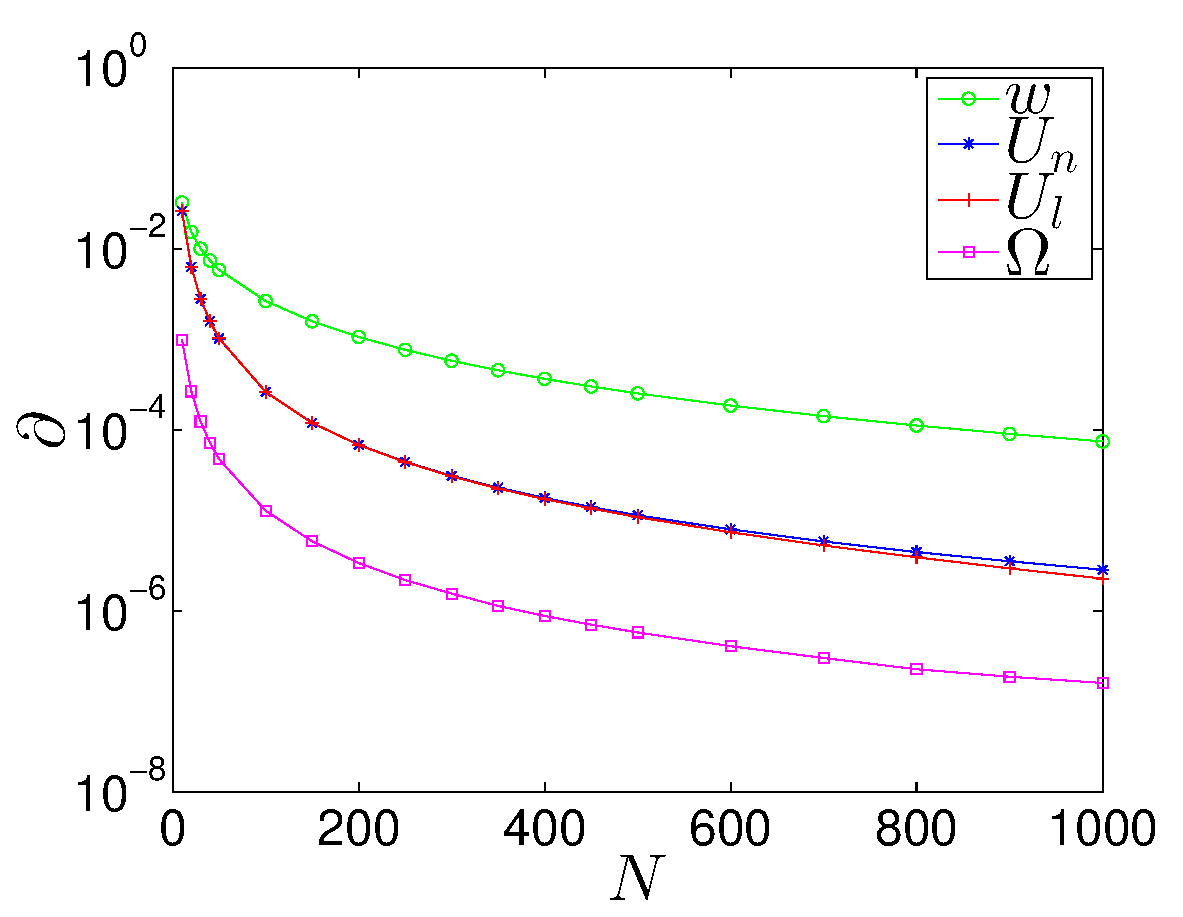
\includegraphics[width=\textwidth]{3_PKN_numerical/accuracy/eps_5_L.eps}
        \end{subfigure}
         \begin{picture}(0,0)(490,-105)
        \put(50,-15){$\varepsilon=10^{-3}$}     \put(200,-85){$\varepsilon=10^{-4}$} \put(380,-15){$\varepsilon=10^{-5}$}
        \put(3,10){a)} \put(168,10){b)} \put(335,10){c)}
        %\put(200,-50){\line(1,1){10}}
        \put(3,-33){$\delta L$}      \put(165,-33){$\delta L$} \put(330,-33){$\delta L$}
        \put(80,-110){$N$}    \put(245,-110){$N$} \put(413,-110){$N$}
        \end{picture}
\caption{Distribution of relative errors of the fracture length $\delta L$ computed by solvers based on different dependent variables ($w$, $U$ and $\Omega$).
When dependent variable $U$ is considered, two different regularised boundary conditions are in use: (\ref{expan_3}) for $U_l$ and (\ref{expan_4}) for $U_n$.
Other parameters are the same as in Fig~\ref{fig:err_N_plots}. Zoom picture within the Fig.~\ref{fig:err_N_plots_L} b) corresponds to the sharp minimum of $\delta L$ for the variable $U_l$.}
\label{fig:err_N_plots_L}
\end{figure*}




\begin{figure*}
        \centering
        \begin{subfigure}{0.32\textwidth}
                \centering
                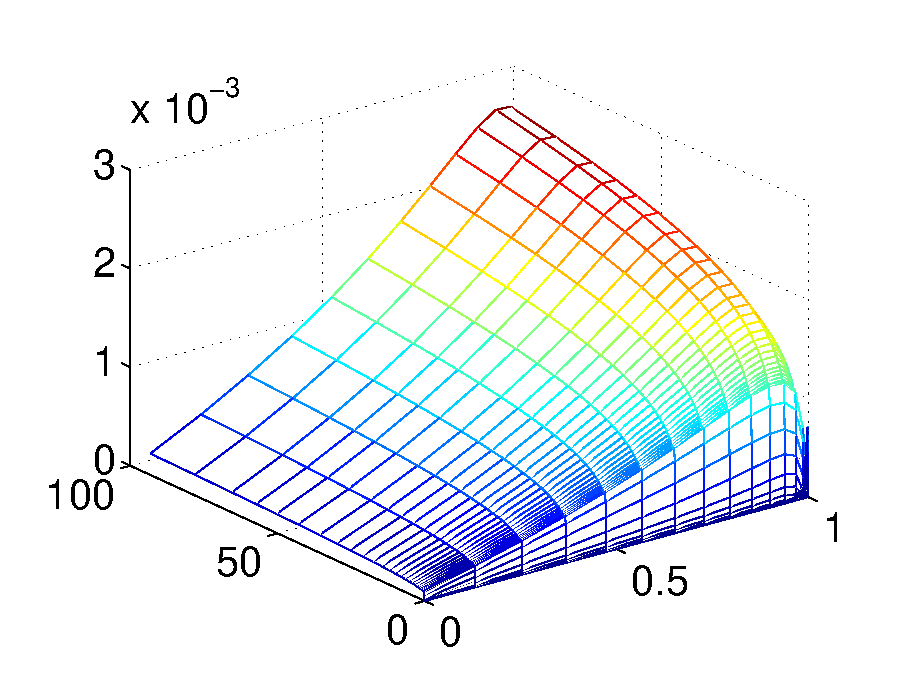
\includegraphics[width=\textwidth]{3_PKN_numerical/accuracy/w_abs.eps}
 \end{subfigure}
 \begin{subfigure}{0.32\textwidth}
                \centering
               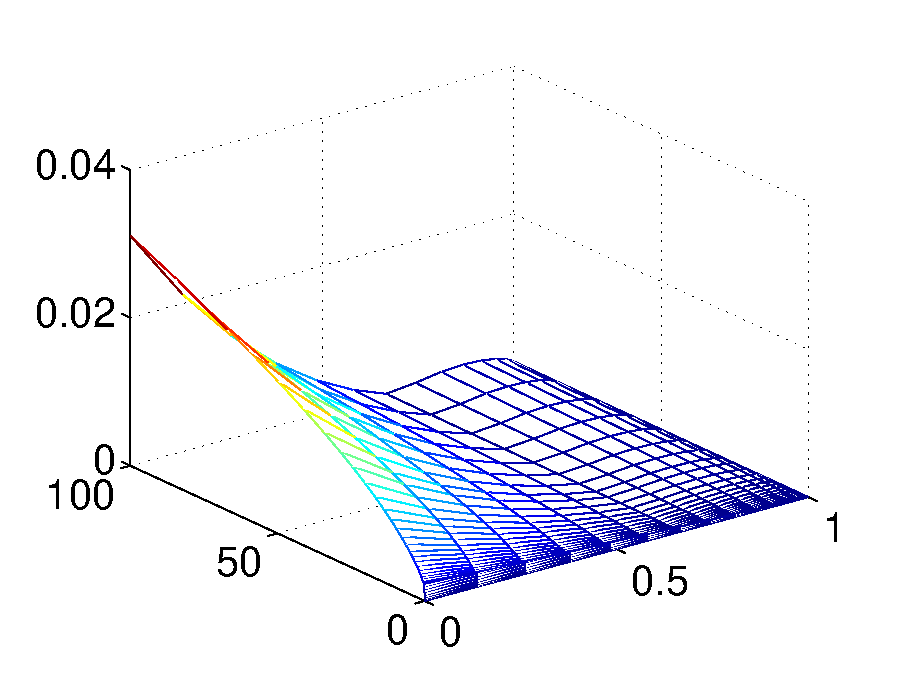
\includegraphics[width=\textwidth]{3_PKN_numerical/accuracy/U_abs.eps}
\end{subfigure}
 \begin{subfigure}{0.32\textwidth}
                \centering
               \includegraphics[width=\textwidth]{3_PKN_numerical/accuracy/Omega_abs.eps}
\end{subfigure}
     \begin{picture}(0,0)(490,-50)%(490,-105)
    \put(30,-95){$t$}     \put(190,-95){$t$} \put(355,-95){$t$}
        \put(3,5){a)} \put(168,5){b)} \put(335,5){c)}
        %\put(200,-50){\line(1,1){10}}
        \put(3,-33){$\Delta w$}      \put(163,-33){$\Delta U_n$} \put(324,-33){$\Delta \Omega$}
        \put(130,-100){$x$}    \put(295,-100){$x$} \put(453,-100){$x$}
        \end{picture}

  \caption{Absolute error for solutions $w$, $U_n$ and $\Omega$ computed for benchmark $q_l^{(1)}$ with ratio $Q_l/q_0=0.9$ and nonuniform mesh $x^{(II)}$ ($\delta=2$) with $N=100$ nodal points. Other parameters: $\varepsilon=10^{-3}$ for $w$, $\varepsilon=5\cdot10^{-3}$ for $\Omega$, and $\varepsilon=10^{-5}$ for $U_n$.}
    \label{distr_total_abs}
\end{figure*}



\begin{figure*}
        \centering
        \begin{subfigure}{0.32\textwidth}
                \centering
                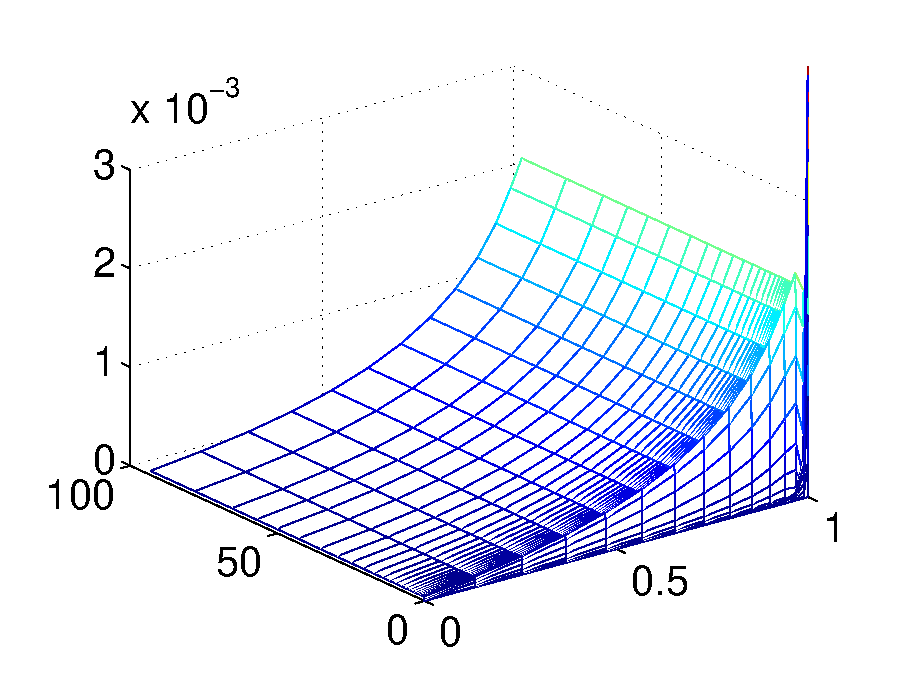
\includegraphics[width=\textwidth]{3_PKN_numerical/accuracy/w_rel.eps}
 \end{subfigure}
 \begin{subfigure}{0.32\textwidth}
                \centering
               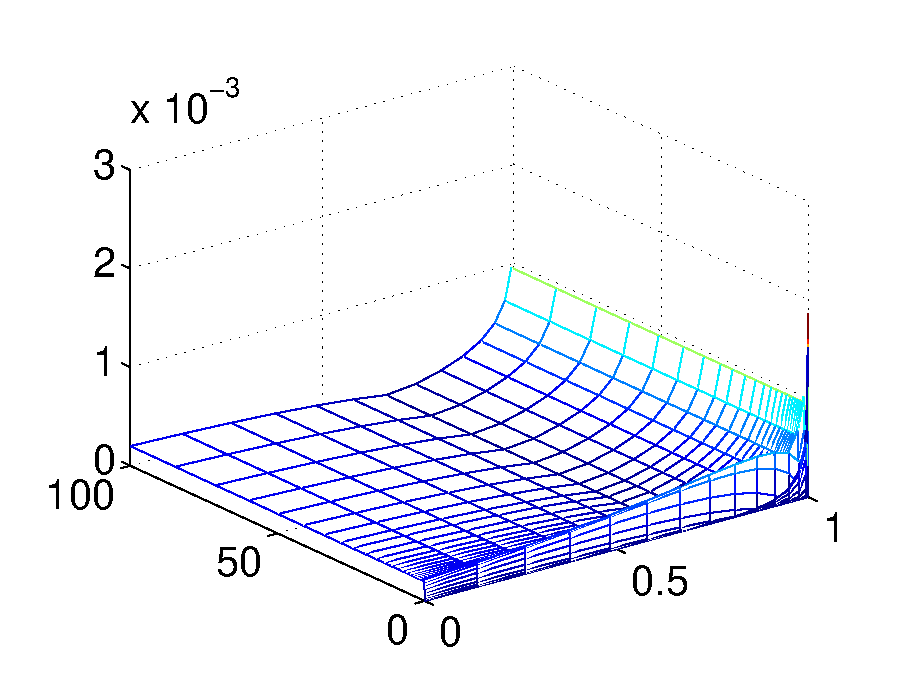
\includegraphics[width=\textwidth]{3_PKN_numerical/accuracy/U_rel.eps}
                \end{subfigure}
 \begin{subfigure}{0.32\textwidth}
                \centering
               \includegraphics[width=\textwidth]{3_PKN_numerical/accuracy/Omega_rel.eps}
                \end{subfigure}
                         \begin{picture}(0,0)(490,-50)%(490,-105)
        \put(30,-95){$t$}     \put(190,-95){$t$} \put(355,-95){$t$}
        \put(3,5){a)} \put(168,5){b)} \put(335,5){c)}
        %\put(200,-50){\line(1,1){10}}
        \put(3,-33){$\delta w$}      \put(163,-33){$\delta U_n$} \put(327,-33){$\delta \Omega$}
        \put(130,-100){$x$}    \put(295,-100){$x$} \put(453,-100){$x$}
        \end{picture}

  \caption{
  Relative error of the solutions $w$, $U_n$ and $\Omega$ computed on the corresponding solvers for the same parameters as in  Fig.~\ref{distr_total_abs}.}
     \label{distr_total}
\end{figure*}





We have not observed any significant difference between the time step strategies chosen by the ode15s solver for the different dynamic systems.
The number of steps and the main trends were similar. For this reason we have not presented any details in the tables.


To visualize the results reported in the Tables \ref{table_w} -- \ref{table_Omega}, and to complement those presented in Fig.~\ref{fig:err_N_plots},
in Fig.~\ref{fig:err_N_plots_L} we show the relative errors of the crack length $\delta L$
computed by different dynamic systems (built on different variables).
The same benchmark and the values of all other problem parameters as previously discussed in Fig.~\ref{fig:err_N_plots} were considered.
If the trends for the different relative errors of the solution $\delta f$ and the crack length $\delta L$ in case of
 $\varepsilon=10^{-3}$ look similar, the results for the smaller value of the parameter are rather surprising. Indeed,
the relative errors $\delta U_l$ and $\delta U_n$ are smaller than $\delta w$ and $\delta \Omega$, while
the error $\delta L$ computed for $U$ no longer follows this trend.

This paradox needs an explanation. A trivial one could be that the maximal error for the solution ($\delta f$) is not situated near the crack tip but inside the computational domain.
To verify this hypothesis and to give a prospective reader a clear picture of the distribution of the solution error in time and space, we present, in  Fig.~\ref{distr_total_abs} and Fig.~\ref{distr_total},
the corresponding absolute and relative errors computed for the nonuniform mesh built on $N=100$ nodal points with the corresponding optimal regularized parameters
discussed after Fig.~\ref{fig:err_N_plots}. As it follows from Fig.~\ref{distr_total}, the maximum of the relative error is always achieved near the crack tip
($\max_{t}\delta f(t,1-\varepsilon))$). Hence, the initial guess has not been confirmed.
On the other hand, the values of the relative errors $\delta f$ and the respective $\delta L^{(f)}$
are directly interrelated. The following analysis identifies this relationship.


\begin{table*}
\centering
\begin{tabular}{c|c|c|c|c|c|c|c|c|}
\cline{2-9}
& \multicolumn{2}{c|}{$\epsilon=10^{-2}$} & \multicolumn{2}{c|}{$\epsilon=10^{-3}$}& \multicolumn{2}{c|}{$\epsilon=10^{-4}$} & \multicolumn{2}{c|}{$\epsilon=10^{-5}$}
\\ \cline{2-9}
& $x^{(I)}$ & $x^{(II)}$& $x^{(I)}$ & $x^{(II)}$& $x^{(I)}$ & $x^{(II)}$& $x^{(I)}$ & $x^{(II)}$
\\ \cline{1-9}
\multicolumn{1}{|c|}{$\delta w$}&1.6e-2&1.6e-2&3.4e-2&2.5e-3&6.8e-2&2.1e-2&--&8.2e-2
 \\ \cline{1-9}
\multicolumn{1}{|c|}{$\delta U_l$}&1.9e-1&1.9e-1&8.2e-2&8.1e-2&1.0e-1&4.3e-2&1.5e-1&2.3e-2
 \\ \cline{1-9}
\multicolumn{1}{|c|}{$\delta U_n$}&4.8e-2&4.8e-2&1.1e-2&6.3e-3&1.9e-2&3.2e-3&2.0e-2&9.1e-3
 \\ \cline{1-9}
\multicolumn{1}{|c|}{$\delta \Omega$}&2.6e-3&5.0e-3&3.0e-3&1.7e-3&3.9e-3&9.9e-3&4.0e-3&3.0e-2
 \\ \cline{1-9}
\multicolumn{1}{|c|}{$\delta L_w$}&2.0e-4&2.6e-4&2.0e-3&1.8e-4&3.4e-3&3.9e-4&--&6.2e-4
 \\ \cline{1-9}
\multicolumn{1}{|c|}{$\delta L_l$}&1.2e-3&1.1e-3&2.7e-4&1.3e-4&7.5e-4&2.8e-4&1.0e-3&3.2e-4
 \\ \cline{1-9}
\multicolumn{1}{|c|}{$\delta L_n$}&2.5e-4&1.2e-4&1.8e-4&2.6e-4&2.5e-4&3.0e-4&2.6e-4&3.2e-4
 \\ \cline{1-9}
\multicolumn{1}{|c|}{$\delta L_\Omega$}&8.1e-7&4.7e-7&1.1e-6&1.1e-6&1.2e-6&1.2e-6&1.2e-6&1.2e-6
 \\ \cline{1-9}
\end{tabular}
\caption{Accuracy parameters for the limiting (critical) variant of the benchmark solution ($Q_l/q_0=0.9857$, $\gamma_v=2.07$)
computed for different meshes composed of $N=100$ nodal points. The blank positions in the table correspond to the case when the solver ode15s could not complete the computations in a reasonable time.}
\label{table_very_bad_benchmark}
\end{table*}




Using (\ref{expan_1}), after some algebra, one has the estimate:
\begin{equation}
\label{estim}
\delta f\approx\delta e_1^{(f)}+(\delta e_2^{(f)}-\delta e_1^{(f)})\frac{e_2^{(f)}}{e_1^{(f)}}\varepsilon^{\alpha_2-\alpha_1}.
\end{equation}
For the benchmark $q_l^{(1)}$ and $Q_l/q_0=0.9$ (see Appendix C) which always provides the worst accuracy in our computations, one can conclude
\begin{equation}
\label{estim_w}
\delta w\approx\frac{1}{3}\delta U\approx\delta w_0+\frac{1}{10}(\delta w_1-\delta w_0)\sqrt[6]{\varepsilon},
\end{equation}
 \begin{equation}
\label{estim_Omega}
\delta \Omega\approx\delta w_0+\frac{8}{90}(\delta w_1-\delta w_0)\sqrt[6]{\varepsilon}.
\end{equation}
Finally, from (\ref{new_speed}) we can derive
 \begin{equation}
\label{estim_L}
\delta L\approx\frac{3}{2}\delta w_0.
\end{equation}
The last relationship has also been verified numerically by evaluating the values of the constant $w_0$ in the postprocessing procedure
using the computed solution ($w$, $U$ or $\Omega$) and the corresponding regularized boundary condition (compare (\ref{expan_1}) and (\ref{BC_N})).

It is clear from relations (\ref{estim_w}) -- \eqref{estim_Omega} that the relative errors of the respective dependent variables
also depend on the quality of approximation of the second term  in the  regularized boundary condition \eqref{expan_1}.
This explains the surprising relationship between $\delta L$ and the respective $\delta f$.



Interestingly, the results presented in Fig.~\ref{fig:err_N_plots_L} show that the value of $\varepsilon$ which provides the lowest relative error, $\delta f$, of the dependent variable $f$
does not necessarily give the best accuracy of the crack length $\delta L$. Moreover, the relation $\varepsilon=\varepsilon_L(N)$ is much more sensitive to the variation of $N$ than  $\varepsilon=\varepsilon_f(N)$.
 Indeed, one can observe sharp minima (see Fig.~\ref{fig:err_N_plots_L} a) and b)) while there is no such phenomenon in the respective graphs for $\delta f$ (see Fig.~\ref{fig:err_N_plots}).
To demonstrate that the peaks are not computational artifacts, we also include a small zoom of the corresponding area of the figure Fig.~\ref{fig:err_N_plots_L} b).

To complete the accuracy analysis, let us consider some critical
regime of  crack propagation. Namely, assume that the leak-off flux
almost entirely balances the volume of fluid injected into the
crack. Indeed, when taking the Carter type benchmark
\eqref{w_0_bench} $b_1=b_2=1$, one obtains the fluid balance ratio
$Q_l/q_0=0.9857$. This gives a very strong variation of the particle
velocity function along the crack length ($\gamma_v=2.07$ - see \eqref{gamma_v}).

In view of the previous conclusion on the  influence of the ratio $Q_l/q_0$
on the solution accuracy (which in fact confirms the observations from
\citet{MWL}), one can predict that the solution error will increase
appreciably in comparison with the figures shown in Tables
\ref{table_w} -- \ref{table_Omega}. In order to verify this
assertion the computations were made for respective dynamic systems
(the system for $U$ was analyzed again  for two forms of the
regularized boundary condition). Both types of meshes, the uniform
and the non-uniform, were utilized, each composed of 100  nodal
points ($N=100$). Four different values of the regularization
parameter $\varepsilon$ , ranging from $10^{-5}$ to $10^{-2}$, were
analyzed. The results of the computations described by respective
accuracy parameters are presented in Table
\ref{table_very_bad_benchmark}. Here, the symbols $\delta U_l$ and
$\delta U_n$ stand for the relative error of $U$ obtained for the
conditions \eqref{expan_3} and \eqref{expan_4}, respectively. The
subscript of $\delta L$ informs us which dynamic system the
corresponding result was obtained for.

The data in the table shows that the solution error increased at least one order of
magnitude, as compared to the values from Tables \ref{table_w} --
\ref{table_Omega}. The lowest deterioration of the solution accuracy
was obtained for $\Omega$, which proves the best overall performance
of the system built for this variable. Especially impressive is its
advantage when comparing the errors of crack length estimation. In
all considered cases $\delta L_{\Omega}$ is at least two orders of
magnitude lower than $\delta L$ for other dependent variables.

In this critical variant of benchmark solution, the non-linear
regularized boundary condition \eqref{expan_4} for $U$ gives, in
most cases, much better performance than its linear counterpart
\eqref{expan_3} (compare with the discussion after the Tables
\ref{table_UUU} and \ref{table_w} -- \ref{table_Omega}). Finally,
the non-uniform mesh seems to be a better choice from the point of
view of accuracy.

In the last test in this subsection we  discuss the sensitivity of
respective algorithms to the variation of the crack propagation
regime. To this end, consider again the benchmark solution
\eqref{w_bench} for the critical value of the ratio
$Q_l/q_0=0.9857$ ($\gamma_v=2.07$). Now, we analyze a range of parameters $\gamma
>-1/3$, motivated by the physical sense of the solution. By changing this value, one
simulates different modes of crack propagation (see Appendix
\ref{app:C}). The non-uniform mesh
composed of 100 nodes nodes was utilized. For each of the
dependent variables an optimal value of the regularization
parameter, $\varepsilon$, was taken: $\varepsilon=10^{-3}$ for $w$,
$\varepsilon=10^{-5}$ for $U$, and $\varepsilon=5\cdot10^{-3}$ for
$\Omega$. The results of the computations illustrated by the relative
errors of the crack length and the maximal relative errors of
corresponding dependent variables are shown in
Fig.~\ref{L_gamma} -- Fig.~\ref{w_gamma}, respectively.

\begin{figure}[h!]
\center
    \hspace{-2mm}
    \includegraphics [scale=0.35]{3_PKN_numerical/accuracy/L_gamma.eps}
\put(-100,-2){$\gamma$}

    \caption{The relative errors of the crack length for different dependent variables as functions of $\gamma$.}
\label{L_gamma}
\end{figure}

\begin{figure}[h!]
\center
    \hspace{-2mm}
    \includegraphics [scale=0.35]{3_PKN_numerical/accuracy/w_gamma.eps}
    \put(-100,-2){$\gamma$}

    \caption{The maximal relative errors of respective dependent variables as functions of $\gamma$.}
\label{w_gamma}
\end{figure}

As can be seen in Fig.~\ref{L_gamma}, for all dependent variables
the crack length error rapidly decreases for $\gamma \to -1/3$.
Indeed, this is the case when $L(t) \sim L_0$. For $w$ and
$U$ solvers, $\delta L$ remains very stable over most of the analyzed
interval. The solver based on $\Omega$ exhibits quite different
behaviour. For $\gamma$ greater than approximately 1.4, the error
decreases to achieve the level of its ultimate accuracy, the same as
for $\gamma \to -1/3$. Depending on the crack propagation regime,
this solver can give up to two orders of magnitude better accuracy
of $L(t)$ than others.

Fig.~\ref{w_gamma} shows, that respective dependent variables
themselves are much less  sensitive to the changes of $\gamma$ that
the crack length. In the considered interval each solver provides a
relatively stable level of accuracy (with\-in the same order of
magnitude).

This test proves that using the solver based on $\Omega$ is
especially  beneficial when dealing with the problems of fast
propagating fractures (large values of $\gamma$).
